\documentclass[12pt]{report}			% Začátek dokumentu
\usepackage{SP}							% Import stylu

\author{Jonáš Havelka}
\title{Neuronová síť}
\date{19. února 2020}
\vedouci{Dr.rer.nat. Michal Kočer}
\place{V Českých Budějovicích}
\skolnirok{2019/2020}
\logo{
\includegraphics[scale=0.75]{logo_gymji.jpg}}

\begin{document}

\mytitlepage						% Vygenerování titulní strany

\prohlaseni{
	Prohlašuji, že jsem tuto práci vypracoval samostatně s vyznačením všech použitých pramenů.
}

\abstrakt{
	\lipsum[1]						% Abstrakt
}{
	\lipsum[1]						% Klíčová slova
}

\podekovani{
	\lipsum[2]						% Poděkování
}

\tableofcontents
\newpage			% Obsah




\chapter*{Úvod}

\lipsum[1]


\part{Teoretická část}

\chapter{Asymptotická notace}

\section{O-notace}
Odkaz v závorkách: \parencite[see][page 900]{einstein}\\
Odkaz: \cite{knuthwebsite}\\
A odkaz pod čarou: \footcite[see][s. 42]{latexcompanion}\\
Dobrý den, ahoj, \gls{atd}\\
Praha, \gls{tj} hlavní město ČR

\section{Abeceda Abeceda Abeceda Abeceda Abeceda Abeceda Abeceda Abeceda Abeceda Abeceda }
\begin{figure}
	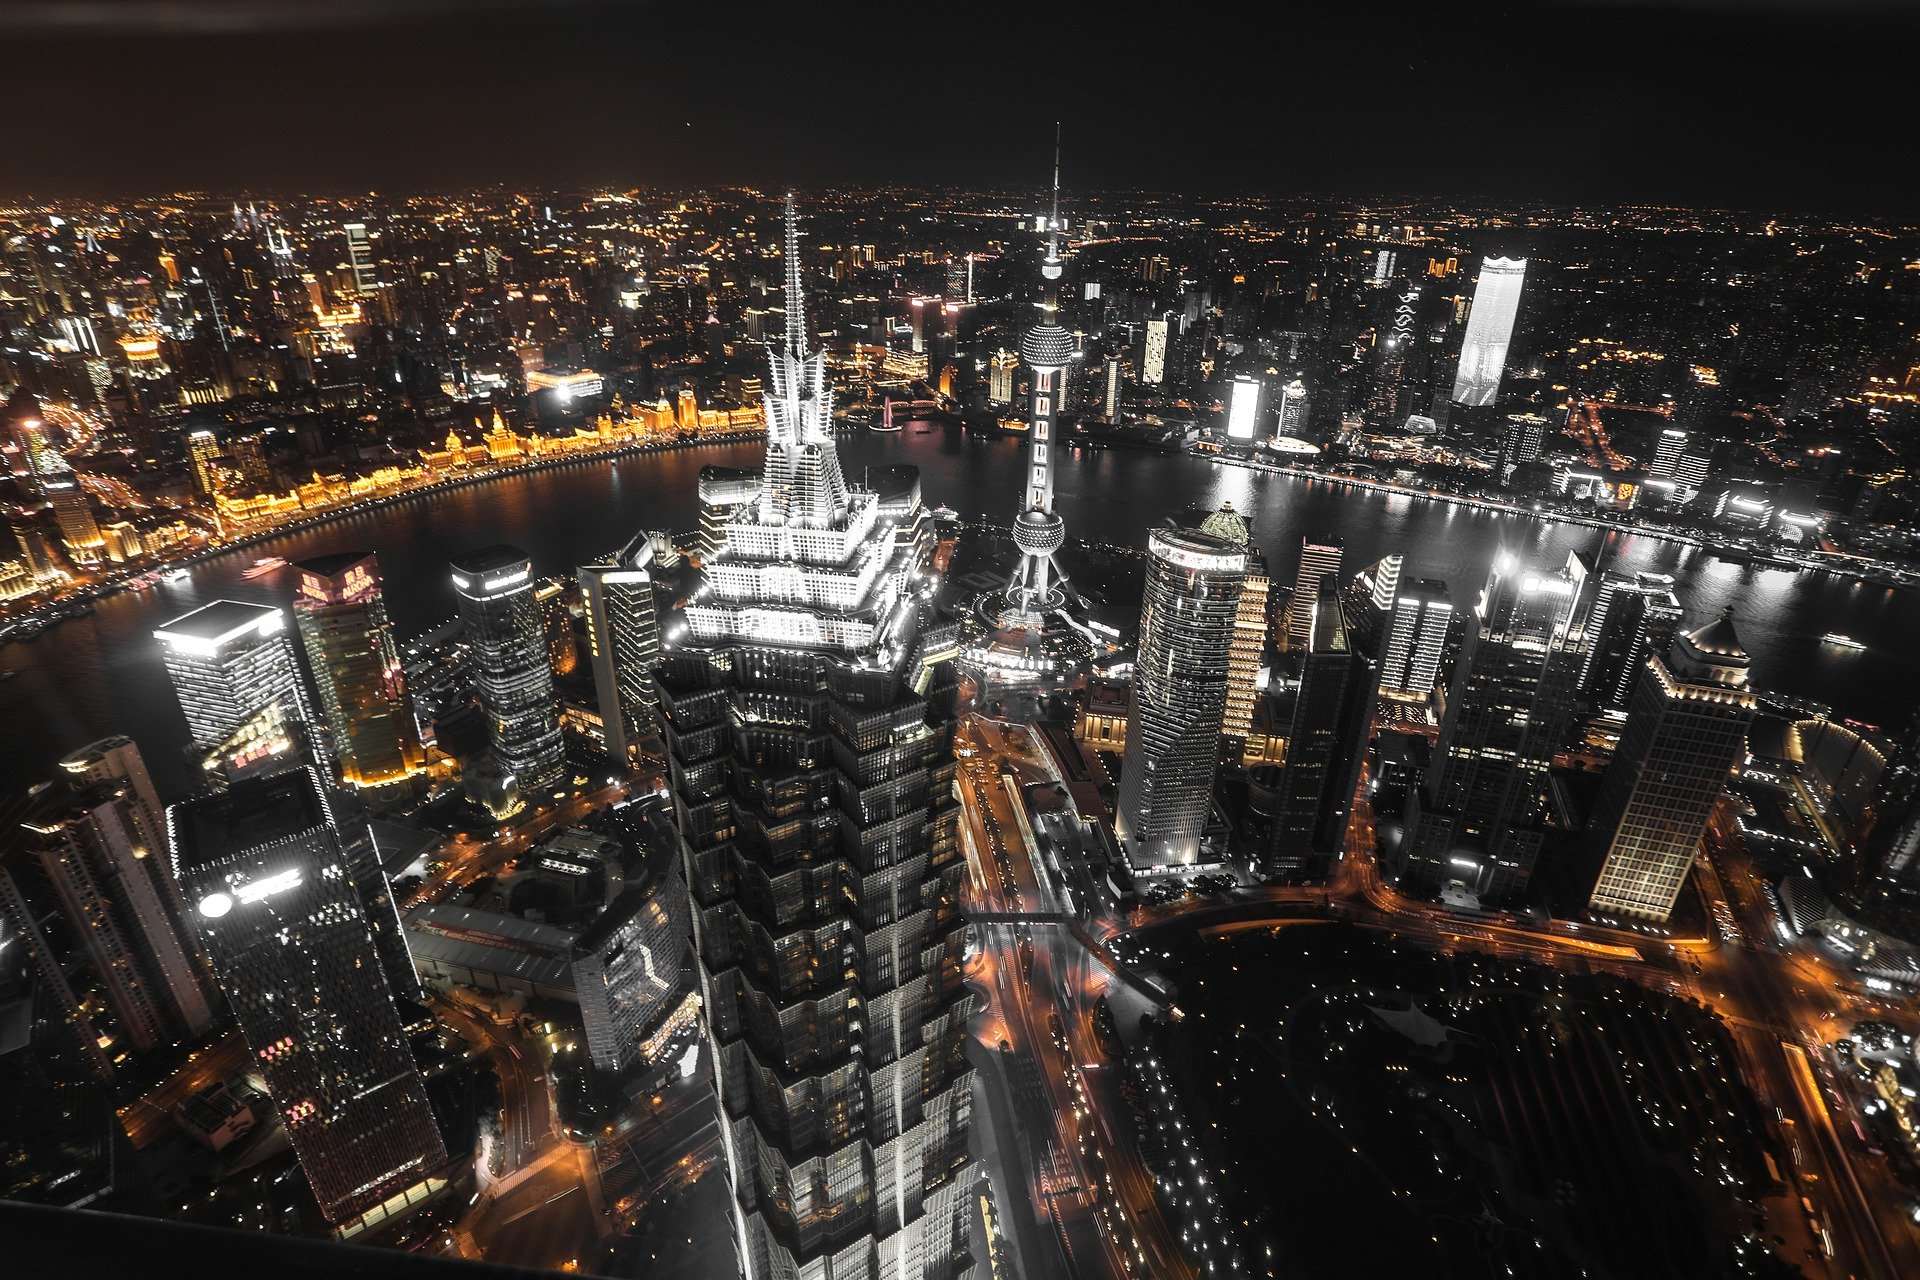
\includegraphics[width=\linewidth]{test.jpg}
	\caption{Testovací}
	\label{fig:test}
\end{figure}
\begin{table}
	\caption{Testovací}
	\label{tab:test2}
	\begin{tabular}{ccccc}
		1 & 1 & 1  & 1  & 1  \\
		1 & 2 & 3  & 4  & 5  \\
		1 & 3 & 6  & 10 & 15 \\
		1 & 4 & 10 & 30 & 45
	\end{tabular}
\end{table}

Obrázek \ref{fig:test} ukazuje Shangai z Pixabay.\\
Tabulka \ref{tab:test2} ukazuje hádejte, co.

\part{Praktická část}



\appendix
\addcontentsline{toc}{part}{Apendix}

\chapter*{Závěr}

\lipsum[1]

\nocite{*}
\printbibliography					% Vytvoří seznam literatury
\addcontentsline{toc}{chapter}{Bibliografie}
\printglossary[title={Zkratky}]		% Vytvoří seznam zkratek
\listoffigures						% Vytvoří seznam obrázků
\listoftables						% Vytvoří seznam tabulek

\begin{prilohy}
	\pitem{Fotky z pokusů}
	\eitem{Vlastní program}
	\eitem{Dokumentace}
	\eitem{Testovací data}
\end{prilohy}
\end{document}